\setstretch{1.5}

\chapter{Estimativa de depósitos minerais}



Este capítulo inicial é uma breve introdução aos conceitos de planejamento mineral e avaliação de recursos e reservas. O objetivo com este texto é iniciar o leitor nos jargões mais comuns da mineração facilitando seu entendimento na utilização da geoestatística em seu meio de trabalho. A estimativa de depósitos minerais é sem dúvida o campo mais importante do uso da geoestatística no setor mineral, lidando com as questões de relevância no planejamento.   

\subsection{Introdução}

Os investimentos necessários para iniciar uma mineração tendem a ser da ordem de grandeza de centenas de milhões de reais. De forma a obter um investimento rentável, o material produzido da mina deve ser potencialmente adequado em quantidade e qualidade necessária para justificar a decisão do investimento.

 A mineração e o processamento mineral devem operar de forma a planejar um lucro aceitável. Certamente todas a tecnologia e as decisões financeiras são tomadas visando a viabilidade do commodite. Logo a estimativa dos teores e a localização do material (reservas in situ) devem ser conhecidas com certo intervalo de segurança. Dessa forma a geoestatística prevalece como o conjunto de metodologias que melhor adéqua as estimativas do depósito mineral.  Apenas garantindo condições de segurança aos investidores externos, por meio de amostragens corretas e cálculos confiáveis é possível atrair investimentos financeiros para o empreendimento mineral. 
 
Isso é de fato verdadeiro em depósitos extensos e disseminados ao qual os teores são apenas ligeiramente acima das condições de lucratividade e para materiais preciosos onde somente existe um percentual pequeno mineralizado que pode ser explotado com certo lucro. 
 
 Os lucros na mineração são altamente nivelados pelo preço de mercado e pelo teor do material minerado. Uma pequena diferença entre os valores planejados e realizados ou uma pequena diferença no preço do metal associado tem um grande impacto na lucratividade da mina. 
 
 Para permanecer competitiva, as companhias de mineração devem otimizar sua produtividade em cada operação unitária. Há várias formas de se conseguir este objetivo. Movimentando ou processando mais toneladas de material com o menos equipamento é uma das alternativas, seguido de um melhor controle das operações ou comprando equipamentos mais eficientes. Todas essas formas de operação estão associadas com um custo e  com um potencial de retorno do investimento. Outra forma de agregar valor ao commodite é potencializando o conteúdo metálico do produto, utilizando rotas de beneficiamento mais eficientes. 
 Os três pilares para o controle das incertezas na mineração e otimização das operações de mineração são: estimativa do minério, planejamento mineral e controle dos teores.
 
 \subsection{Estimativa dos depósitos mienrais}

Jazidas minerais são consideradas uma quantificação formal da ocorrência de materiais naturais, que são estimados por uma variedade de procedimentos tanto epíricos como teóricos. Estas são consideradas a base do estudo de viabilidade econômica  e são classificadas como reservas e recursos. Considera-se uma reserva mineral quando apenas estima-se possíveis quantidades de material capazes de gerar um lucro para o empreendimento. Já um recurso mineral é uma quantidade limitada que possui um nível de confiança suficiente para garantir lucratividade, disponibilidade técnica, jurídica, ambiental e social. 

Os recursos e reservas minerais são determinados a partir de amostras de rochas que determinam um volume de rocha mineralizado de uma ordem de grandeza muito maior do que o volume da amostra. Esses erros de estimativa são vistos como erros de extensão ao considerar a ampliação dos valores da amostra para o todo. Com o objetivo de caracterizar um depósito mineral este é dividido em um conjunto de blocos, ao qual o valor estimado de cada bloco está relacionado com os dados mais proximais. Logo a jazida mineral pode ser vista como um quebra-cabeça de blocos com tamanhos individuais, localização e teores estabelecidos.

A quantificação de recursos e reservas minerais exige um certo grau de confiabilidade (subjetivo ou estatístico) apropriado para os dados disponíveis durante a estimativa. Volumes, massa, teores e quantidades de metal ou minerais são atributos geralmente quantificados. A estimativa deve ser otimizada tal que deve ser não enviesada e erro não deve ultrapassar um critério de qualidade. 

 \subsection{Alguns conceitos iniciais sobre jazidas minerais}
 
 Na engenharia de mina, tal como na estimativa de depósitos minerais e planejamento mineral, há uma série de jargões técnicos utilizados. É importante compreendê-los de forma a planificar o entendimento sobre o assunto tratado. Maiores informações sobre conceitos básicos de pesquisa mineral podem ser encontrados em \cite{sinclair2002applied} 
 
\subsubsection{Minério} : 

Minério é uma rocha ou mineral que é extraído por trabalhos de mineração com o intuito (mesmo que algumas vezes não alcançado) de obter vantagens para a comunidade. Dentre estas vantagens pode-se citar o benefício econômico, a produção exclusiva para construção civil, a obtenção de recursos energéticos para  o Estado ou na pesquisa científica.

O termo minério é aplicado a rochas em três formas mais comuns. 1) Como uma descrição econômica, relacionada com o controle de qualidade das reservas minerais e com o seu conteúdo 2) Como um commodite vendido à parte do seu conteúdo, tal como em pedras de construção 3) Ou como um material fragmentado oriundo de uma mina. 

O primeiro tópico é o de  maior importância e implica na distinção de minério (material minerado com lucro) e estéril (que não contêm valor suficiente para se obter lucro). A definição de minério e estéril é uma função dependente do tempo que relaciona diversos fatores tais como preço, tecnologia, regime de taxação, condições ambientais, sociais, etc. 

Em geral minas são colocadas em atividade com o entendimento que será possível um retorno necessário ao seu investimento. As circunstâncias ditarão a concepção do preço e consequentemente daquilo caracterizado como minério e estéril. 

Para reduzir os efeitos da incerteza do tempo um a mineração geralmente trabalha antecipadamente com três formas de planejamento, a curto, médio e longo prazo. 

\subsubsection{Teor de corte}

O conceito de teor de corte ou cutoff é definido como aquele em que o valor do conteúdo metálico ou mineral em um certo volume de rocha começa a atender as especificações econômicas da mina. Os teores de corte são usados para distinguir blocos de minério e estéril em vários estágios da evolução da estimativa da jazida mineral (exploração, desenvolvimento e produção). Minério/Estéril são baseados nos valores estimados. Em alguns os erros de estimativa podem levar à uma classificação errada do material. A figura \eqref{Grafico_validacao} demonstra quatro regiões definidas pelos erros de estimativa. O material classificado como minério pode ser estéril ou de fato minério, enquanto o material classifcado com estéril pode ser minério ou  de fato estéril.   

\begin{figure}[H]
	\centering
	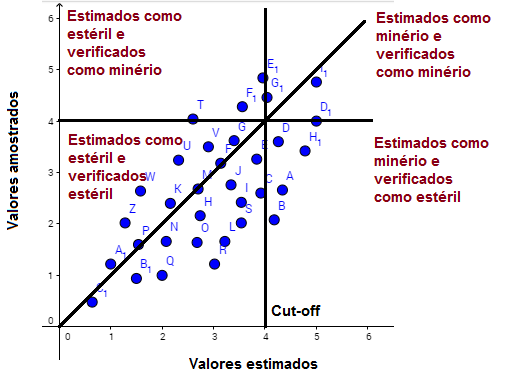
\includegraphics[scale=1.0]{grafico_aderencia.png}	
	\caption{Figura demonstrando o gráfico de aderência entre os valores estimados e verificados posteriormente por amostragem. Quatro regiões determinadas pelo valor de teor de corte }
	\label{Grafico_validacao}
\end{figure}

Com o aumento do teor de corte, a massa de minério tende a diminuir e o teor médio da jazida acima do teor de corte tende a aumentar. Geralmente com o aumento da razão estéril e minério ( unidades de estéril a ser removido por unidade de minério retirado) também aumenta com o teor de corte. Geralmente apenas um pequeno espectro de teores de corte são considerados no processo de simulação e seleção de um cenário particular de mineração. 

O conceito de teor de corte também está ligado com a conectividade dos minérios durante o estágio de produção. Com o aumento do teor de corte o volume de minério tende a se dividir de forma a criar volumes separados na jazida. 

A estimativa do teor de corte é na verdade um problema econômico complexo, e está fora do escopo deste libro, no entanto podemos apresentá-la de forma simplificada. 

O custo operacional de um minério por tonelada beneficiada pode ser dado por \eqref{custo_operacional}

\begin{equation}\label{custo_operacional}
OC = FC + (SR +1 )MC
\end{equation}

Em que FC é o custo fixo, SR é a relação estéril minério e MC é o custo de mineração por tonelada movimentada. 

O fluxo de caixa de um mina pode ser dado pela relação \eqref{Fluxo_caixa}

\begin{equation}\label{Fluxo_caixa}
CF = Receita - Custos operacionais = (g.F.P-OC)T
\end{equation}

Onde g é o teor médio do minério, F é o fator de recuperação da metalurgia e P é a recuperação do metal por tonelada beneficiada e T a tonelagem de material beneficiado. Logo podemos encontrar o teor de corte quando o Fluxo de caixa é igual a zero \eqref{Fluxo_caixa2} 

\begin{equation}\label{Fluxo_caixa2}
g = \frac{OC}{F.P}
\end{equation} 

\subsubsection{Continuidade}

Continuidade pode ser definido como o grau de conectividade no espaço. Na avaliação de depósitos este termo é utilizado ambiguamente como uma ocorrência física ou natural geológica, tal como uma estrutura, um litotipo ou uma mineralização ou como o grau de correlação espacial entre variáveis aleatórias. Um capítulo neste livro é dedicado somente a caracterização da continuidade estatística de variáveis aleatórias.

\subsubsection{Diluição}

A diluição é o resultado da mistura do minério com estéril durante o processo de produção, geralmente causando um aumento do volume de material retirado e decréscimo do valor médio do teor segundo as expectativas. Pode-se dividir a diluição em duas categorias: interna ( material de baixo teor envolvido de material com alto teor ) ou externa (material de alto teor envolvido com material de baixo teor). 

\subsubsection{Recursos e reservas minerais}

Jazidas geralmente são consideradas em termos de recursos ou reservas minerais. As definições geralmente variam segundo uma jurisdição para outra, no entanto há um grande esforço para tornar os conceitos internacionalizados. Na falta de consenso internacional, há uma tendência tando industrial como técnica de adotar o código australiano ou JORC(Joint Ore Reserves Committee).

Um recurso é uma ocorrência mineral quantificada alicerçado nos dados geológicos e no teor de corte simplesmente. Diversas são as formas de se classificar os recursos minerais, sejam elas baseadas simplesmente na geometria das amostras, na variância de krigagem ou em simulações geoestatísticas. Na maioria dos códigos não existe metodologias prescritas primordialmente. Espera-se apenas que se utilize um critério que garanta confiabilidade nas estimativas. Os recursos são subdivididos em medido, indicado e inferido segundo o grau de confiabilidade das medidas. Essas classificações podem ser feitas segundo uma distância geométrica do centro da amostra, de intervalos para o valor da variância de krigagem em uma região ou para um nível de confiabilidade para a distribuição de uma parcela do depósito mineral. Espera-se que o valor medido tenha maior confiabilidade, o indicado menor e o inferido pouca certeza.
  

Recursos podem ser transformados em reservas minerais caso haja um estudo de viabilidade do depósito mineral. Este incorpora uma variedade de aspectos relacionados com a lucratividade do bem mineral e estão ligados com as questões ambientais , técnicas, sociais, jurídicas e financeiras do empreendimento. As reservas são dividas em provável e provados. 

A classificação das regiões do depósito são variáveis ao longo do desenvolvimento do projeto e das fases de desenvolvimento da mina, devido ao acréscimo de informação. Um recurso pode se tornar uma reserva mineral e vice-versa. A figura \eqref{Recursos_Reservas} demonstra a transição das diversas classificações. 

\begin{figure}[H]
\centering
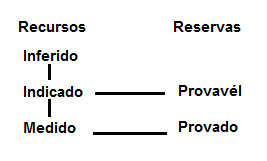
\includegraphics[scale=1.0]{Recursos_Reservas.png}	
\caption{Figura demonstrado a classificação de jazidas em recursos e reservas. Linhas indicando a transição entre as classificações }
\label{Recursos_Reservas}
\end{figure}

\subsubsection{Unidade Seletiva de mineração}

Uma unidade seletiva de mineração é o menor bloco ao qual se define um material como minério ou estéril, ou seja, o menor volume de rocha no planejamento capaz de ser retirado e decidido sua finalidade, seja para a usina de beneficiamento, seja para a pilha de estéril. O tamanho da unidade seletiva de mineração depende do método de lavra utilizado e da escala de produção da operação. Para objetivos de planejamento um depósito mineral pode ser considerado um arranjo de blocos definidos por esta unidade, cada um com seu valor associado de teor e outros parâmetros como densidade, massa, volume, saturação de água, etc. 

Na decisão do tamanho de bloco duas condições são impostas para a determinação do seu volume. A primeira são as condições operacionais da mineração, tal como altura do talude, volume a ser retirado com o caminhão, dimensão da malha de desmonte, espaçamento durante a produção e etc. A segunda é o tamanho mínimo para uma estimativa confiável. Esta geralmente é calculada como 1/4 da distância média entre as amostras. A sub-blocagem, ou seja, a divisão dos blocos para atender os requisitos operacionais não deve ser feita durante a fase de estimativa, mas apenas sobre os blocos estimados, como forma de adequar o processo à operação. 

\subsubsection{Precisão e Exatidão}

Exatidão pode ser exemplificado como a proximidade de uma estimativa com a realidade, enquanto precisão é a medida da dispersão entorno de uma estimativa. Uma estimativa pode ser exata, mas não precisa, ou precisa, mas não exata. A figura \eqref{exat_prec} demonstra os conceitos de exatidão e precisão a partir de figuras de alvos. O centro do alvo é o valor verdadeiro que pretende-se alcançar com os disparos. Disparos entorno do centro são considerados exatos, enquanto disparos próximos aos outros são considerados precisos. 

\begin{figure}[H]
\centering
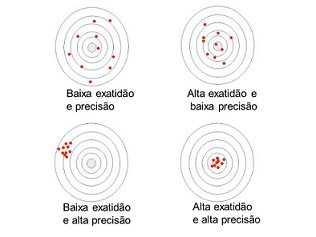
\includegraphics[scale=1.0]{exat_prec.jpg}	
\caption{Figura demonstrando os conceitos de exatidão e precisão. O centro do alvo é o valor verdadeiro que pretende-se alcançar com os disparos. Disparos entorno do centro são considerados exatos. Disparos próximos aos outros são considerados precisos }
\label{exat_prec}
\end{figure}

Na estimativa de depósitos minerais é natural que os nossos disparos não sejam precisos, mas é mais que importante que sejam exatos. Não é admitido obter valores médios com erros deslocados da média global. Isto também é chamado de viés ou deriva. 

Há vários tipos de erros potenciais na estimativa de reservas minerais incluindo:

\begin{itemize}
\item Erro de amostragem 
\item Erros de análise química.
\item Erros de densidade (É comum em muitos casos considerar a densidade do material constante ao longo do depósito)
\item Erros da geologia, durante as fases de determinação da continuidade espacial e geometria do depósito mineral.
\item Na escolha do método de lavra adotado que pode não atender as questões de seletividade do minério e estéril de forma ótima.
\item A diluição do minério com a encaixante.
\item Erro humano (inserção de valores errados no banco de dados, de casas decimais, et.)
\item Fraude ( salgamento de amostras, substituições de amostras, dados não representativos, etc.)

\end{itemize}

\section{Softwares de Mineração}

Durante a fase de avaliação das jazidas minerais o computador exerce função essencial como ferramenta de estudo. Uma quantidade substancial de softwares estão disponíveis em meio comercial e alguns aplicativos livres também existem. Softwares comerciais são mais onerosos, mas possuem suporte técnico e manutenção de seus sistemas. Apresentam código fechado ao público externo pertencente geralmente ao proprietários. Softwares gratuitos geralmente são disponibilizados por universidades, possuem código aberto ao público e podem ser facilmente obtidos via Internet.  

Uma das bibliotecas gratuitas mais importantes é sem dúvida o GSLIB (Geostatistical Software Library) e apresenta além dos executáveis do programa seus algoritmos, escritos em fortran 90 e disponibilizados no site. Os programas são administrados pelo doutor Clayton Deutsch e Emmanuel Schnetzler. Mais informações sobre o pacote de softwares pode ser encontrado no site www.gslib.com ou no guia de uso \cite{deutschcv1998gslib}

O uso dos softwares de mineração geralmente requerem que os arquivos de dados sejam organizados eficientemente em formatos pré-estabelecidos, gerados pelas campanhas de exploração.  Essa compilação dos dados é trabalhosa e necessita de uma validação primordial, tornando o trabalho de preparação dos dados às vezes muito mais demorado que várias implementações dos programas.  

Entre as aplicações mais comuns encontradas em softwares de mineração relacionadas com a estimativa de depósitos temos:

\begin{itemize}
\item Uma grande variedade de procedimentos de avaliação dos dados (estatísticas, gráficos, etc.:)
\item Determinação da qualidade dos dados e dos protocolos de amostragem
\item Modelagem tridimensional e visualização de formas geológicas complexas e distribuição das amostras.
\item Preparação de seções planas e verticais 
\item Gráficos de contorno tanto do teor como de outras variáveis 
\item Caracterização da continuidade espacial (Variogramas automáticos, mapas de variograma, variogramas experimentais e modelagem)
\item Modelagem de blocos do depósito
\item Metodologias de cálculos de recurso e reservas
\item Avaliações dos efeitos de vários métodos de mineração
\item Determinação da viabilidade econômica de depósitos
\end{itemize}

Alguns destes softwares podem ainda incluir ferramentas de planejamento de mina, tal como otimização de cava, sequenciamento, desenho de cava, etc. 

A grande desvantagem da maioria dos softwares, principalmente dos pagos é algumas questões referentes ao seu funcionamento que não são explicadas pelos manuais. Alguns modelos matemáticos, são de fato, "escondidos" dentro das rotinas dos programas. Isso dificulta a tomada de decisão dos operadores em alguns casos e pode até ser prejudicial em algumas formas. 


